\section{イントロダクション}

本資料は2025年に大谷・末原研究室(仮名)\footnote{
これまで森・大谷研究室と呼んでいたので筆者には少し違和感があるが、時期慣れるだろう。
}に入る学生が少しでも早く研究室に慣れるために用意した。大谷・末原研の研究室メンバーや研究内容に関して紹介する。


\section{プロジェクト紹介}

\subsection{ILC計画}
aaa
\subsection{US-Japanカロリメータ開発}
aaa
\subsection{MEG II実験}
aaa
\subsection{次世代$\mu^{+}\rightarrow e^{+}\gamma$探索実験}
aaa
\subsection{PIONEER実験}
aaa
\section{メンバー紹介}
aaa
\subsection{大谷航准教授}
aaa

\begin{figure}[h]
  \centering
  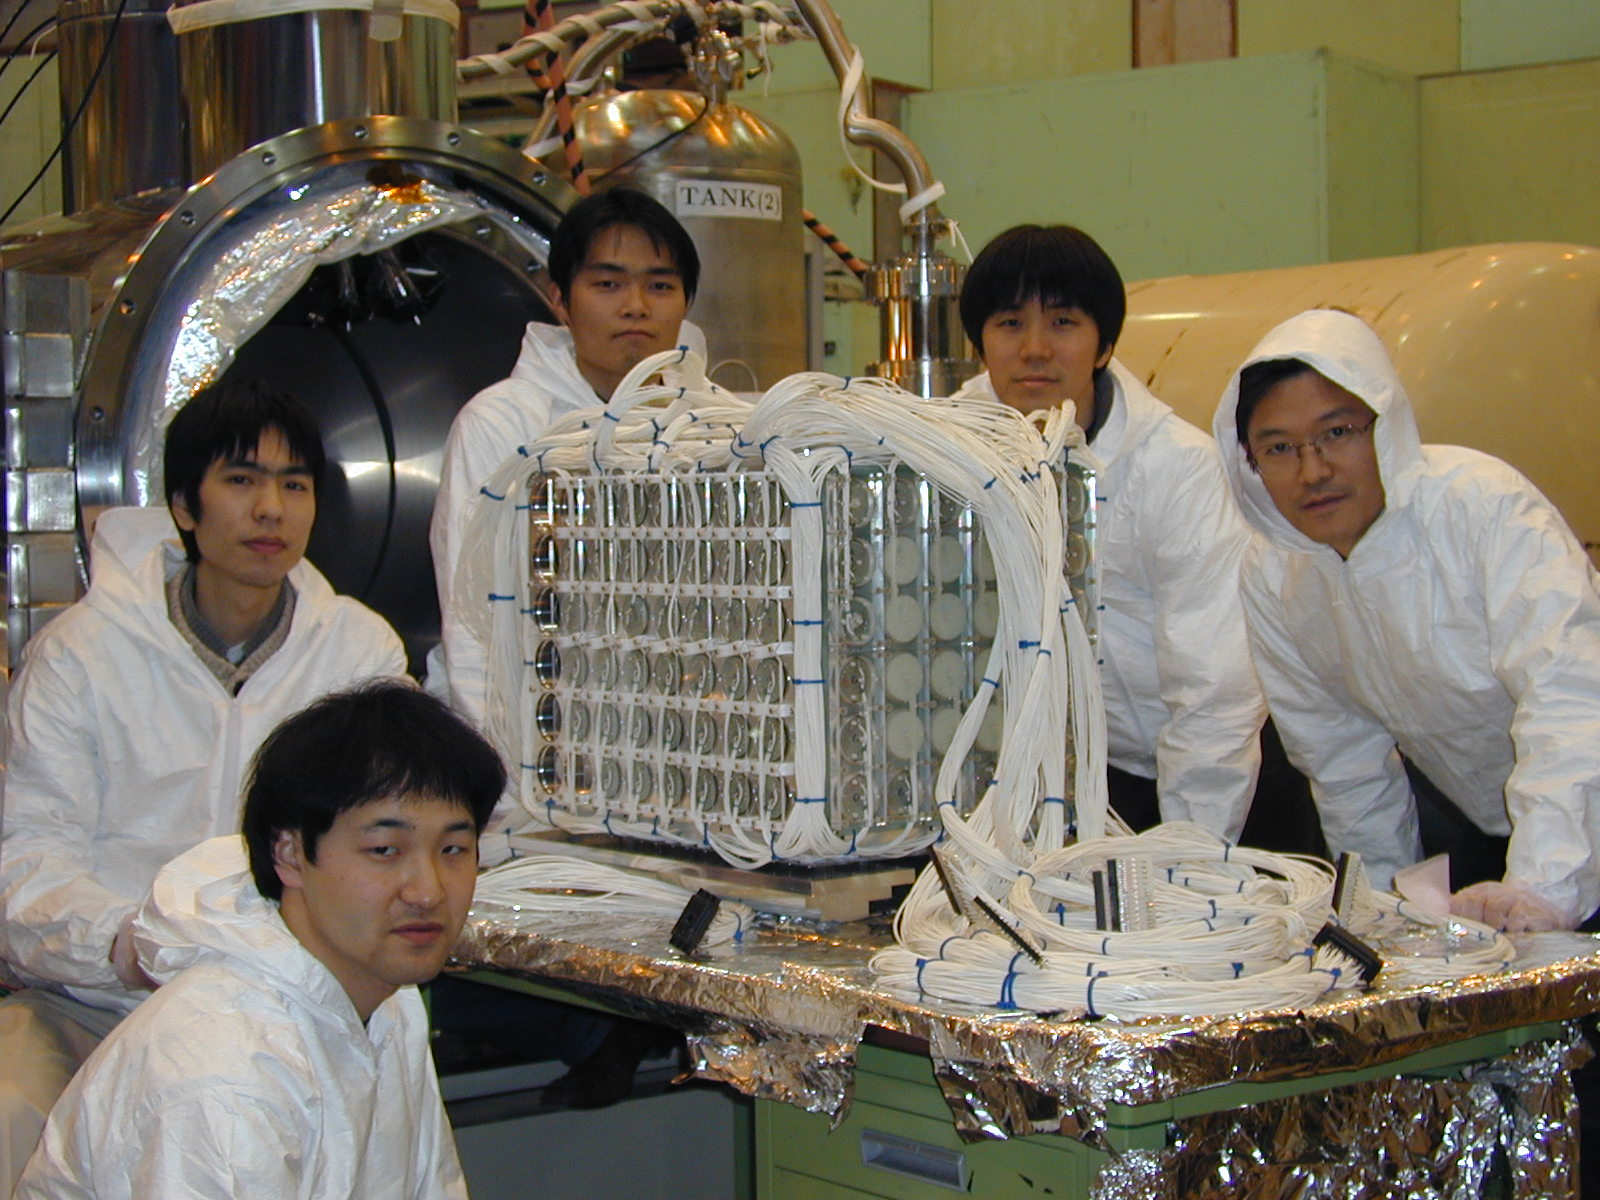
\includegraphics[width=0.9\columnwidth,clip]{fig/wataru.jpg}
  \caption{Large prototypeと呼ばれるMEG II液体キセノン検出器の試作器を試験する大谷さんたち。右から三原さん、大谷さん、西口さん、澤田さん、あと名前わからない人。三原さんと西口さんは現在KEKの研究者で、澤田さんは(ご存知の通り)ICEPPの研究者である。}
  \label{fig:wataru}
\end{figure}


%% \begin{figure}[h]
%%   \centering
%%   \begin{subfigure}[t]{0.45\columnwidth}
%%     \centering
%%     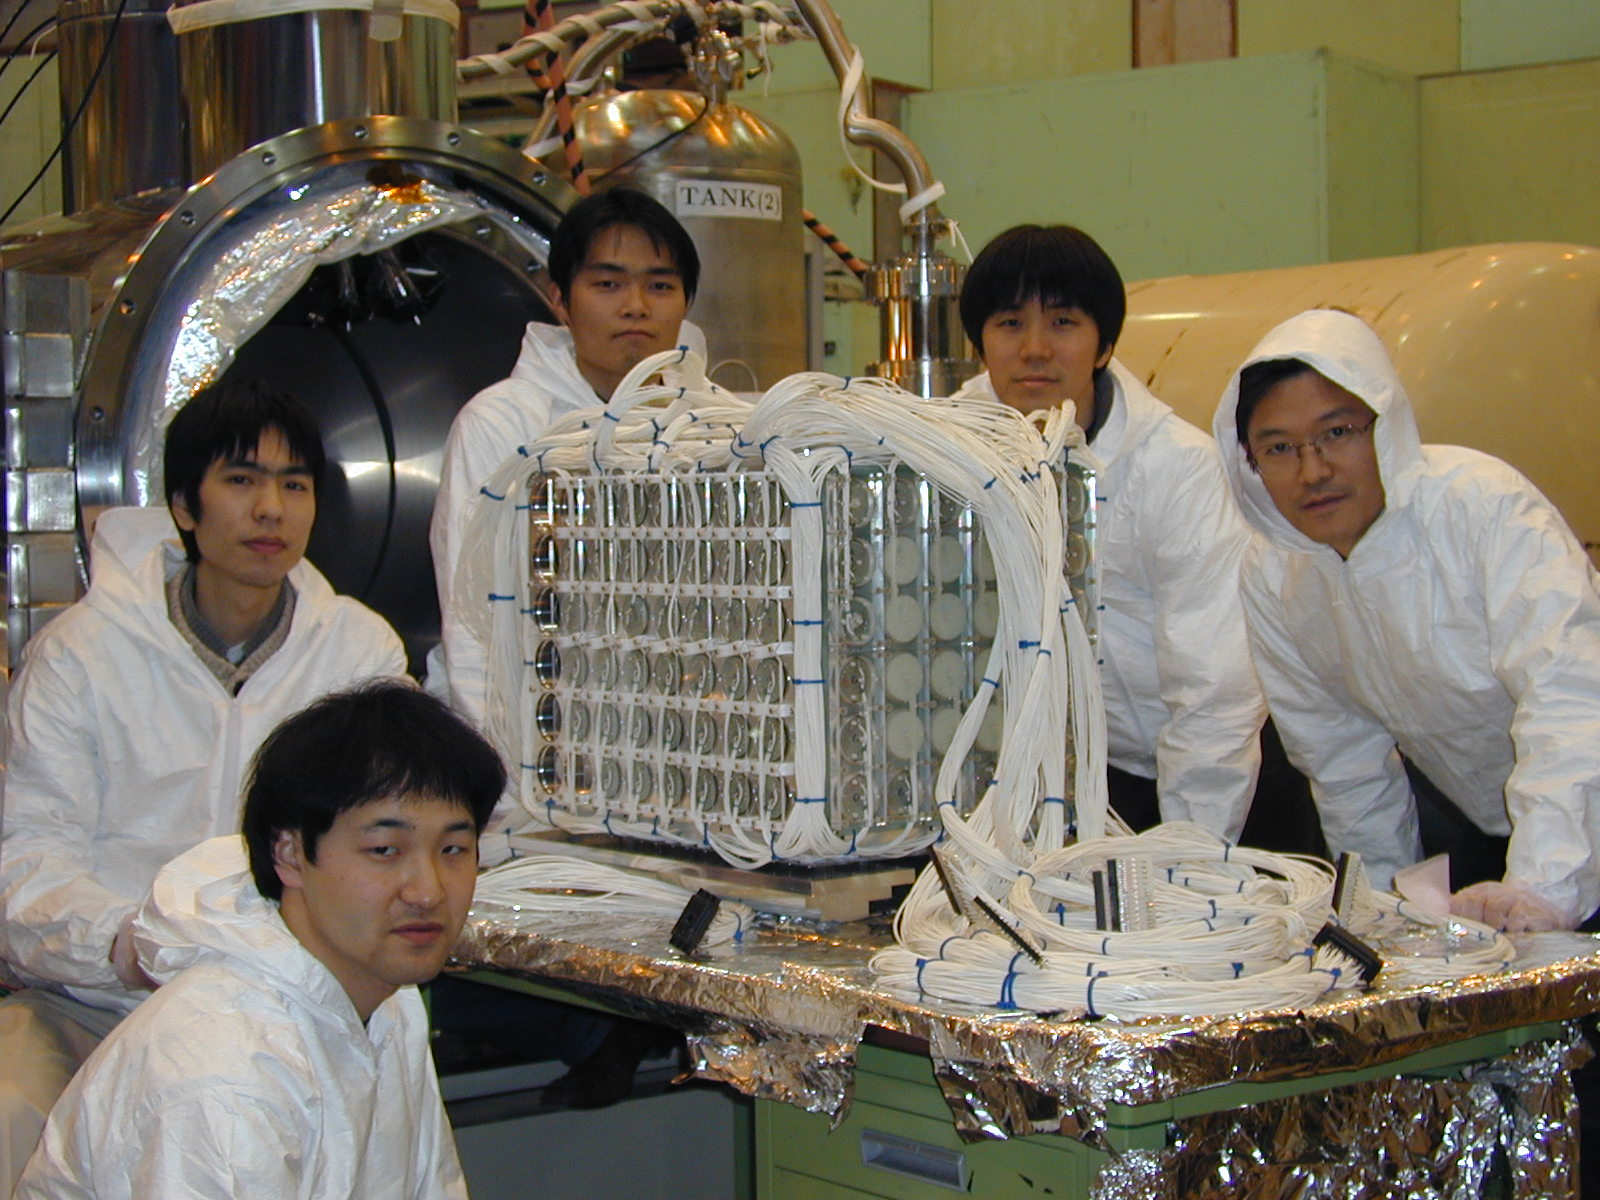
\includegraphics[width=\columnwidth,clip]{fig/wataru.jpg}
%%     \caption{}
%%     \label{fig:wataru}
%%   \end{subfigure}
%%   \hspace{0.1\columnwidth}
%%   \begin{subfigure}[t]{0.45\columnwidth}
%%     \centering
%%     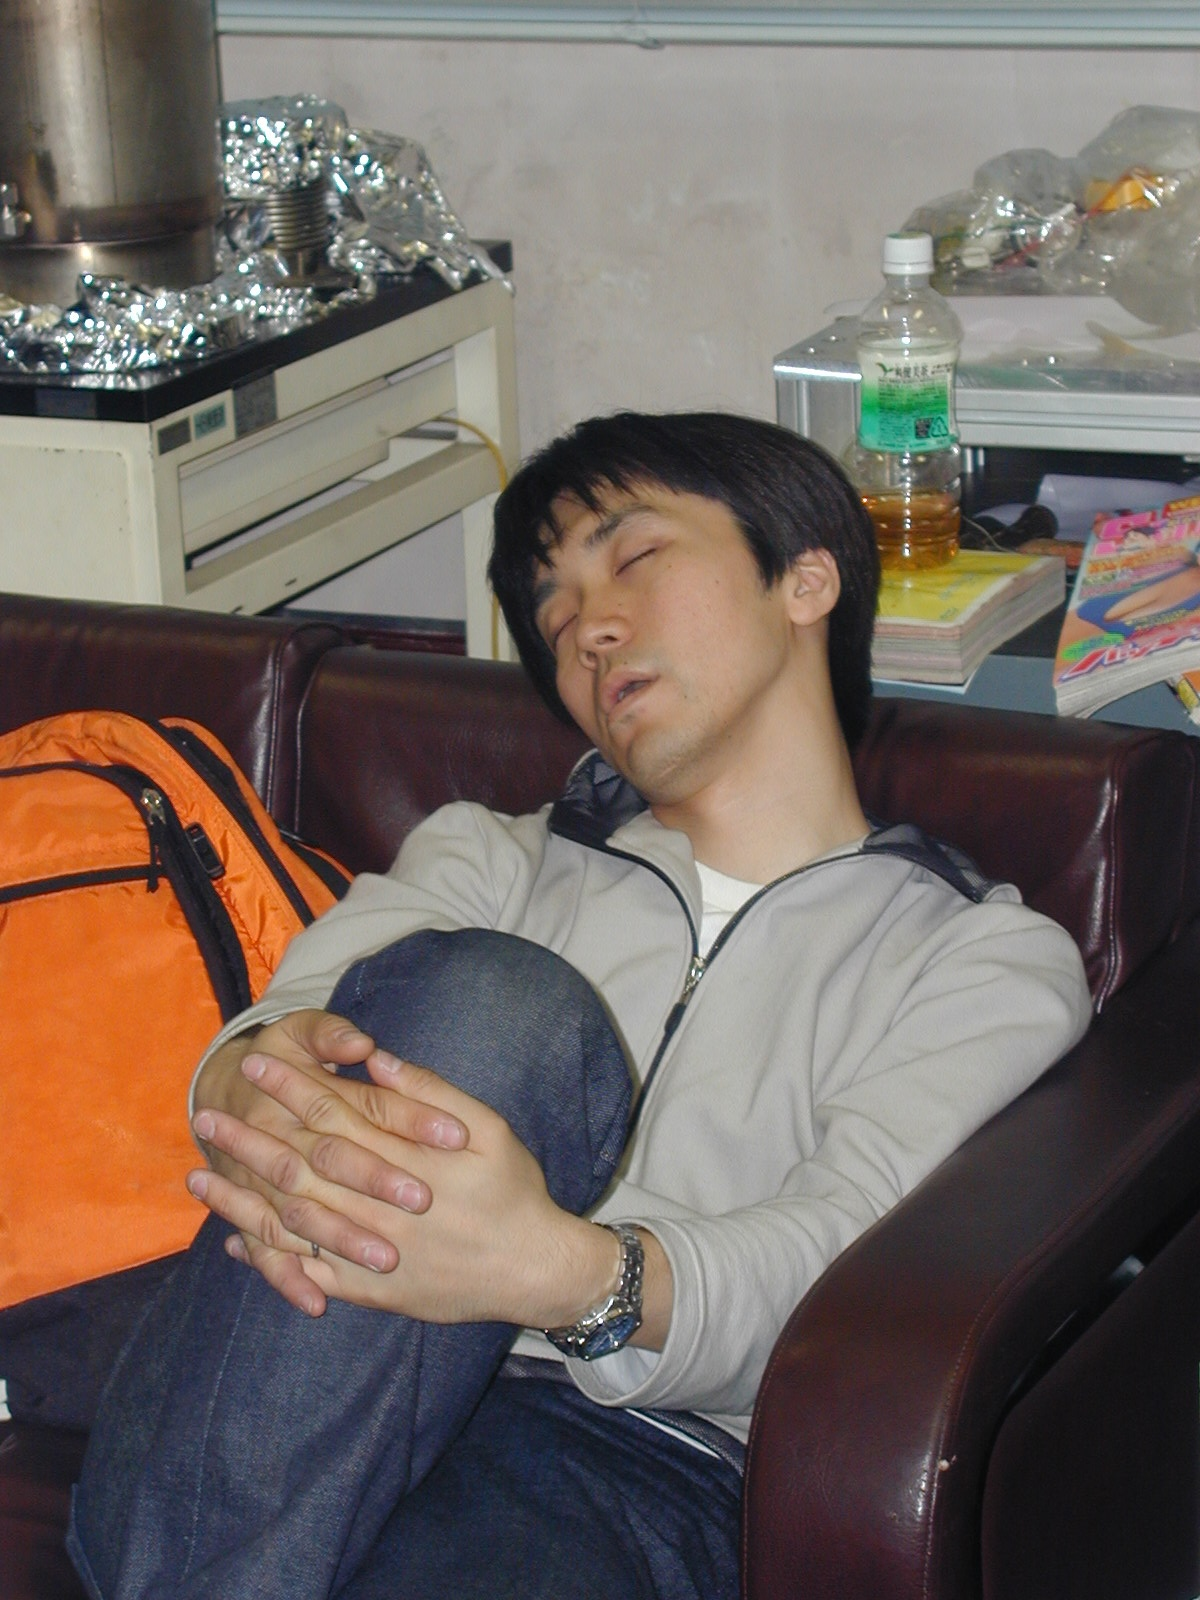
\includegraphics[width=\columnwidth,clip]{fig/wataru_sleeping.jpg}
%%     \caption{}
%%     \label{fig:wataru_sleeping}
%%   \end{subfigure}
%%   \caption{}
%%   \label{fig:wataru_summary}
%% \end{figure}


\begin{wrapfigure}{R}{0.3\columnwidth}
  \vspace*{-\intextsep}
  \centering
  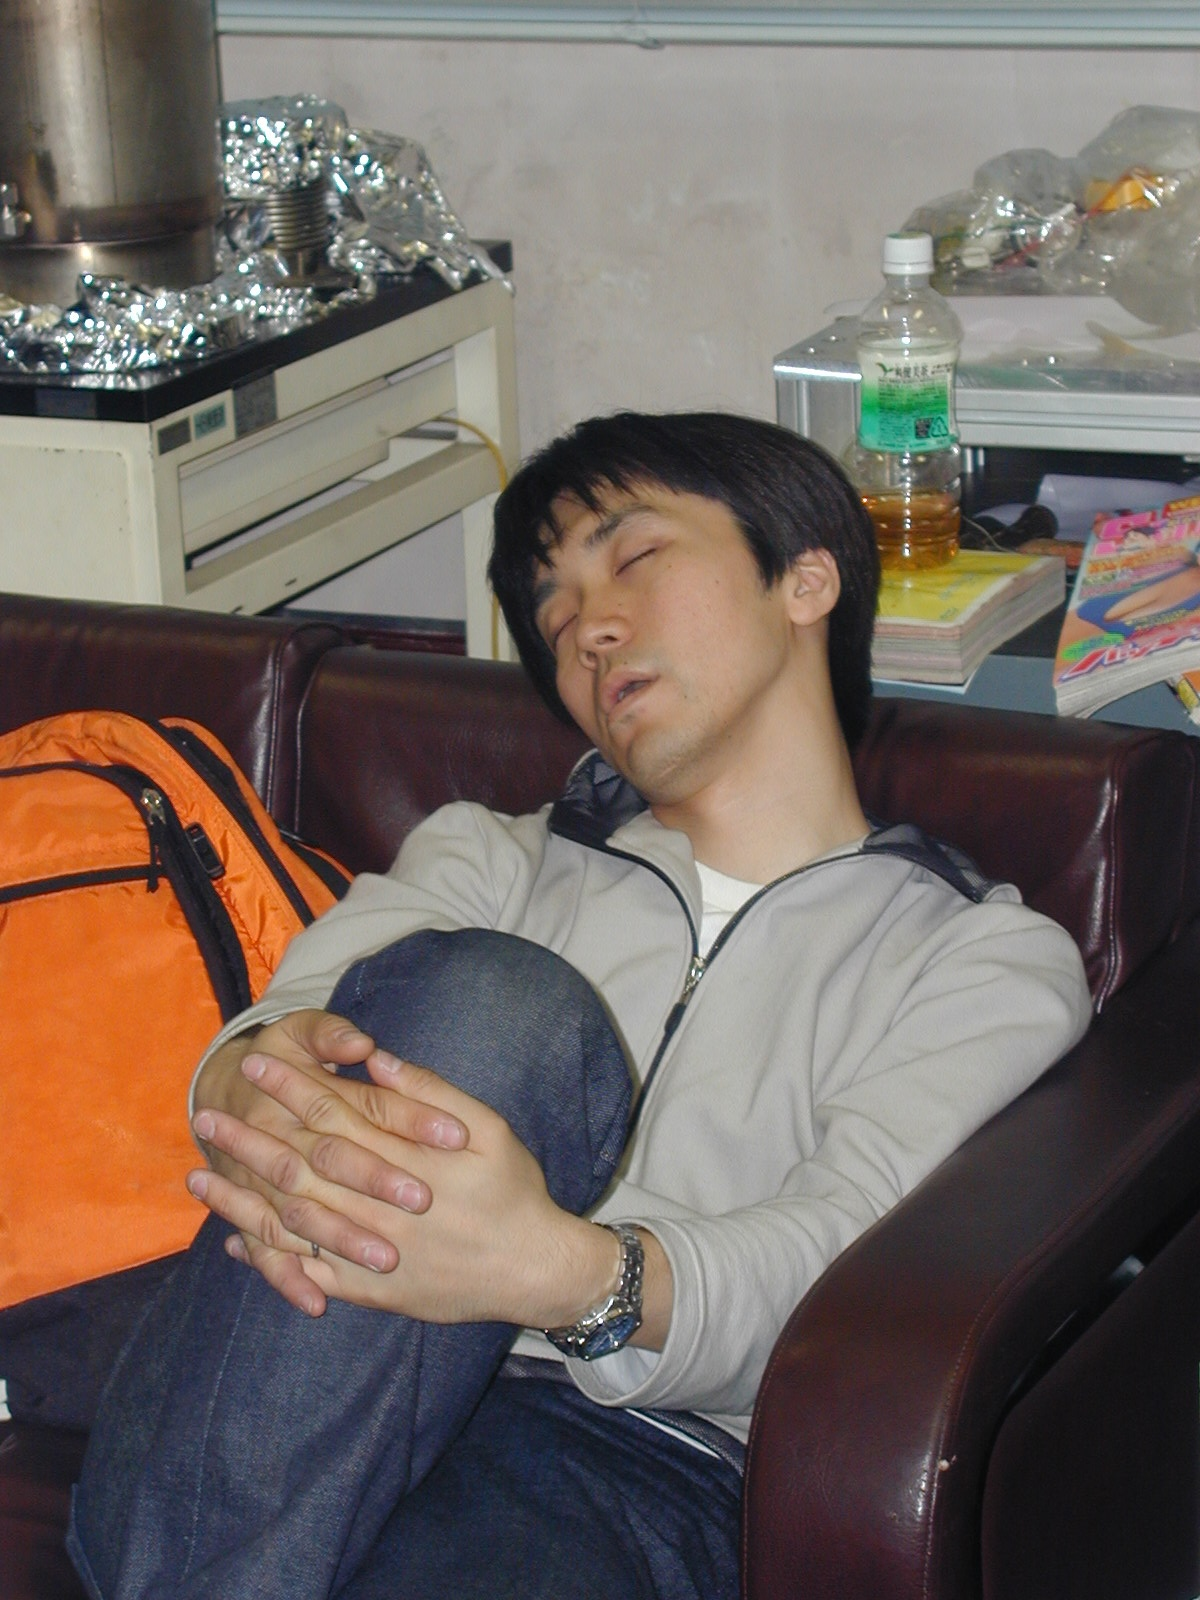
\includegraphics[width=0.3\columnwidth]{fig/wataru_sleeping.jpg}
  \caption{研究で疲れ果てて仮眠を取る若かりし頃の大谷さん。}
  \label{fig:wataru_sleeping}
\end{wrapfigure}


\subsection{岩本敏幸助教}
aaa
\subsection{Lukas Gerritzen特任助教}
aaa
\subsection{潘晟特任助教}
aaa
\subsection{大矢淳史特任助教}
aaa
\subsection{山本健介(D4)}
aaa
\subsection{村田樹(D4)}
aaa
\subsection{池田史(D3)}
aaa
\subsection{李維遠(D2)}
aaa
\subsection{馬越隆成(D1)}
aaa
\subsection{小川拓泰(D1)}
aaa
\subsection{神山大樹(D1)}
aaa
\subsection{高津大誠(D1)}
aaa
\subsection{榊原澪(M2)}
aaa
\subsection{清野拓己(M2)}
aaa

